\section{Linearization, persistent components, and tops}
\label{sec:linearization}

We work on one normalized attempt with root \(R\), for one fixed leaf of
the localization identity in Proposition~\ref{prop:localization}.
The estimates will be uniform over its leaves.  All trees, lists, and
collections in this section are finite.  Interval norms are normalized,
whereas norms without an interval subscript use Lebesgue measure.

This section constructs the linear sides required in
Section~\ref{sec:sides} and the core data used in
Section~\ref{sec:counting}.  We expand each matched column once and
inherit its mode labels, while freezing its coefficients over blocks
of dyadic depths.  The PRE and CURRENT frequency graphs separate
the linear side from the core and give the square bound in
Equation~\eqref{eq:src-17}.  Hereditary representative labels and their first
actual-use cells reaching a fixed amplitude threshold, called tops,
then give the pathwise count in Equation~\eqref{eq:src-28}.

We write \(D_{\mathrm m}\) for a main-catalog budget and enlarge it by fixed
powers when necessary:
\[
 \log D_{\mathrm m}\le k^{O(1)}.
\]
This budget covers main-column counts, their coefficient bounds and
inverse private weights, and the multiplicity of relevant groups and
actual uses along a path.  The dimension of the horizontal parameters
of a vertex or of two vertices together is at most
\(d_{\max}\le k^{O(1)}\); we take \(d_{\max}\ge2\).
As before, a factor
\[
 G_0=\exp\bigl(\log^{O(1)}(2k)\bigr)
\]
is a small overhead.  Its value can increase from one estimate to the
next.  It must be distinguished from a fixed power of \(P\).

\subsection{The data retained from localization}
\label{subsec:linearization-data}

We specify the properties of the localization construction used here.
In a fixed basic-\(B\) role \(l\), its output at depth \(s\) has the form
\[
 Z_{l,G,s}=\overline L_{l,G,s}\,\mathcal B_{l,s}B_{l,s},
\]
as in Equation~\eqref{eq:src-14}.  The outer operator is an average of
main ball projections of one fixed rank.  Each individual projection
family is nested in depth.  The product \(\mathcal B_{l,s}\), including
the constituent projections in \(B_{l,s}\), is a fixed signed sum of
averaged products of \(O(\log\mathcal L)\) nested main projection
families, independent of \(G\).  Every coefficient choice in these
averages is fixed across time.

We use the following conclusions of the preceding constructions.
First, columns and ball-mask matches are inherited along a path, and a
matched main column has a short path to the primary center of its
group.  The endpoint version of Lemma~\ref{lem:weyl} and
Lemma~\ref{lem:chart-expansion} therefore apply at its first match.
Second, an endpoint cell with a nonempty ball mask can be retained
whenever it has a downstream actual-use certificate.  The whole
usable-range spaces of distinct groups of the fixed color satisfy
Lemma~\ref{lem:usable-bessel}.  This statement concerns the spans of
main columns on the entire endpoint cells, including all repetitions
of such cells; it is stronger than a separation statement only at
actual uses.  Third, all the endpoint projections and shared histories
are among the column families covered by Lemma~\ref{lem:compression}.
Their column budgets are \(D_{\mathrm m}\), rather than the larger mode
budget introduced below.

These properties also hold on the nested extensions past stopping
boundaries used to define the original summands.  We keep entire input
endpoint cells when applying a projection; only its output need be
restricted to branches with a downstream certificate.

\subsection{A single expansion at the first match}

Choose a dyadic integer \(K\), whose size will be specified below.
Partition the depth schedule of the attempt into blocks
\([b,b+K)\), and set
\[
 u_b=b-4K,\qquad v_b=b-2K,\qquad t_b=b+K.
\]
Let \(r_s\) be the interval length at depth \(s\).  In a basic-\(B\)
role freeze \(Z_{l,G,u_b}\), and set it to zero if \(u_b\) precedes the
attempt.  Positive ball masks and their histories are evaluated at
these pre-depths even when the group has no actual use there.
We retain a \(v_b\)-cell \(J\) for this purpose only when a descendant
actual use of \(G\) occurs in the block.  Basic-\(U\) roles are not
linearized.
Figure~\ref{fig:depth-blocks} records these depths and the common test cell.

\begin{figure}[t]
 \centering
 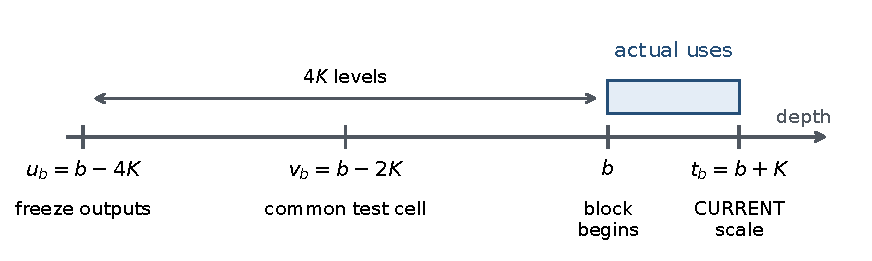
\includegraphics[width=.95\linewidth]{figures/depth-blocks.pdf}
 \caption{A block \([b,b+K)\) of dyadic depths.  Depth increases
 to the right and spatial scale decreases.  Coefficients are frozen
 at \(u_b=b-4K\).  The PRE and CURRENT graphs defined below are both
 evaluated on the same \(v_b=b-2K\) cell, using comparison scales
 \(r_{v_b}\) and \(r_{t_b}\), respectively, where \(t_b=b+K\).
 Each primary's first-match expansion is inherited unchanged across
 blocks.  The counting blocks in Figure~\ref{fig:counting-blocks}
 use a different partition.}
 \label{fig:depth-blocks}
\end{figure}

Fix a group \(G\), with primary center \(z\), and a basic-\(B\) role
\(l\).  A \emph{primary} in this discussion is an individual main
column \(\Phi\) available to the maximal pad of this role's outer ball
filter.  Distinct linear shifts of one vertex tag are distinct
primaries.  At its first match, on a cell \(I_0\), make one expansion
choice and retain that choice on every relevant descendant of \(I_0\).
The lists of primaries and their modes are therefore nested.  Separate
first-match branches may have separate expansions and private labels.
In particular, nothing in an already chosen mode list is resampled at
a later freezing time.

Choose an integer \(Q_0\), common to the roles of this group and within
the main budget, clearing the denominators of \(C_z\), and put
\(\vartheta=\theta_z/Q_0\).
For a uniformly random branch offset \(\rho\) on the unit cube, set
\[
 d^\rho(y)=\rho+\{\theta_z y-\rho\},\qquad
 p^\rho(y)=\lambda_z y^2+(\theta_z y)^T C_zd^\rho(y).
\]
The braces are coordinatewise fractional parts.  Choose a product
Gevrey cutoff \(\zeta^\rho\), periodic in \(\theta_z y-\rho\), with
\(0\le\zeta^\rho\le1\), vanishing within distance \(\delta_c\) of a
coordinate cut and equal to one outside distance \(2\delta_c\), where
\[
 \delta_c=\exp(-k^{C_c}).
\]
The exponent \(C_c\) is fixed sufficiently large after the main
budgets.  Translation invariance of the offset gives
\[
 \E_\rho\zeta^\rho(y)=c_\zeta\ge\tfrac12,\qquad
 \E_\rho|1-(\zeta^\rho(y))^2|^2
       \le C d_{\max}\delta_c
\]
at every \(y\).  A zero-dimensional horizontal parameter has the
constant convention \(\zeta^\rho=1\).
For each role and group the offset will be common to every branch and
time, and independent of the already completed main selections.

\begin{lemma}[First-match expansion and bounded lift]
\label{lem:first-match-lift}
At each first match \(I_0\), there is a finite, permanently labeled
expansion
\[
 \zeta^\rho(y)\varphi_\Phi(y)e(-c_l p^\rho(y))
 =\sum_m a_{\Phi,m}e(\lambda_m y^2+\gamma_m y)
       +O(\delta_c),\qquad y\in I_0,
\]
where all the modes belonging to this primary have the same
\(\lambda_m\).  We may use augmented mode atoms
\begin{equation*}
 \psi_m(y)=
 \left(
 \zeta^\rho(y)e(c_l p^\rho(y))
       e(\lambda_m y^2+\gamma_m y),
 \ \epsilon_{\mathrm m}^{1/2}\mathbf e_m
 \right).
 \tag{20}\label{eq:src-20}
\end{equation*}
Their private indices distinguish primaries and first-match
expansions.  For an admissible budget \(D_1\), with
\(\log D_1\le\operatorname{poly}(P,k)\), we have
\[
 |\lambda_m|\,|I_0|^2\le D_1,\qquad
 \sum_m|a_{\Phi,m}|\le D_1,
\]
and the number of modes is at most \(D_1\).  For two modes of this
primary,
\begin{equation*}
 \gamma_m-\gamma_{m'}=a\cdot(\theta_v,\vartheta),
 \qquad a\in\Q^{\dim(\theta_v,\vartheta)}
       \text{ has height at most }D_1 .
 \tag{21}\label{eq:src-21}
\end{equation*}
There is a block-independent pointwise linear operator
\(\mathscr R_{l,G}\), of uniformly bounded norm, mapping each frozen
outer ball output to exactly the corresponding synthesis of
Equation~\eqref{eq:src-20}.
\end{lemma}

\begin{proof}
The branch cutoff makes the conjugating factor a smooth quadratic
chart supported in a bounded branch cube.  At \(I_0\), the joint
difference data of \(v\) and \(z\) obey the endpoint version of
Equation~\eqref{eq:src-2}, with the harmless fixed factor \(c_l\).
Recenter at \(I_0\), choose one rational splitting there, and apply
Lemma~\ref{lem:chart-expansion}.  Its tail estimate gives the stated
uniform error and finite coefficient and count bounds.  A single
splitting gives a single effective quadratic coefficient for this
primary.  Recentring adds a common unrestricted linear shift; the
differences of the remaining linear shifts are rational combinations
of the two endpoint horizontal vectors.  Clearing \(Q_0\) gives
Equation~\eqref{eq:src-21}.  All these choices are made once.

Here is an explicit lift, which will also explain its operator
properties.  Write the main atom as
\(\Phi=(\varphi_\Phi,\epsilon_\Phi^{1/2}\mathbf e_\Phi)\), and set
\[
 q_\Phi(y)=
 \sum_m a_{\Phi,m}(\psi_m)_{\phys}(y)
       -(\zeta^\rho(y))^2\varphi_\Phi(y).
\]
It satisfies \(|q_\Phi|\le\delta_c\) on the matched subtree.
For a main augmented input \(F\), define the physical part of
\(\mathscr R_{l,G}F\) by
\[
 (\zeta^\rho)^2 F_{\phys}
 +\sum_{\Phi\ {\rm matched\ at}\ y}
       \frac{F_\Phi(y)}{\epsilon_\Phi^{1/2}}q_\Phi(y).
\]
Its mode coordinate \(m\), belonging to \(\Phi\), is
\[
 \epsilon_{\mathrm m}^{1/2}a_{\Phi,m}
       \frac{F_\Phi(y)}{\epsilon_\Phi^{1/2}},
\]
and is zero before the appropriate match.  The main count and inverse
weight bounds, followed by Cauchy--Schwarz, bound the physical
correction's pointwise operator norm by
\(\delta_c D_{\mathrm m}^{C}\).  Choose
\(\epsilon_{\mathrm m}>0\) so small that the squared norm of the
mode-coordinate map is bounded by one.  The preceding count and
coefficient estimates allow
\(\log(1/\epsilon_{\mathrm m})\le\operatorname{poly}(P,k)\).
Thus the whole lift has a uniform pointwise norm.

An outer ball output on a cell has a representation
\(\sum_\Phi\beta_\Phi\Phi\) with constant coefficients, including when
the projection is averaged.  Its main private coordinate is exactly
\(\epsilon_\Phi^{1/2}\beta_\Phi\).  Substitution in the displayed
definition gives
\(\sum_{\Phi,m}\beta_\Phi a_{\Phi,m}\psi_m\), as required.
The lift is pointwise and hence cell-local; it has not been commuted
through any projection.
\end{proof}

Put
\[
 \widetilde Z_{l,G,b}=\mathscr R_{l,G}Z_{l,G,u_b}
\]
on the retained branches.  It is a mode sum
\(\sum_m\alpha_m\psi_m\), with coefficients constant on the
\(u_b\)-cell.  Its available list may include every primary matched
for the maximal pad and rank, whether or not its coefficient is zero.
Fix a budget
\[
 D_*\ge e^k,\qquad \log D_*\le\operatorname{poly}(P,k),
\]
large enough for all the preceding mode counts, rational heights,
coefficient sums, inverse private weights, and \(Q_0\).
It also bounds the total number of available modes over all relevant
groups along a path, all actual cell/group uses, and the sums
\(\sum_m|\alpha_m|\) in normalized frozen evaluations.  These bounds
follow from the main coefficient bounds and
Lemma~\ref{lem:first-match-lift}; groups with a certified nonempty
endpoint already have historical data on that path.  We use disjoint
private coordinates to place all the required spaces in one Hilbert
space.

\subsection{The common progression multiplier and parameter order}

The common gauge has an additional property needed in the core
estimate.  Allow four different offsets \(\rho_j\), and let
\(y_j=y_0+jt\).  On the supports of their four cutoffs,
\(\prod_j e(c_jp^{\rho_j}(y_j))\) agrees with a smooth periodic
multiplier in
\((\vartheta y_{l'},\vartheta t)\), for any anchor \(l'\).  This
multiplier can be chosen bounded by one.

To verify this, write \(d_j=d^{\rho_j}(y_j)\).  Each
\(d_j-\theta_z y_j\) is an integer vector, so
\[
 k_j=d_j-(1-j)d_0-jd_1
\]
is an integer vector.  It is bounded, and locally constant away from
the branch cuts.  The identities
\(\sum_jc_j=\sum_jjc_j=\sum_jj^2c_j=0\) cancel the quadratic terms and
the terms containing \(d_0,d_1\), leaving
\[
 \prod_j e(c_jp^{\rho_j}(y_j))
   =e\!\left(\sum_jc_j(\theta_z y_j)^TC_zk_j\right).
\]
For each fixed carry choice the right side is an ordinary character
on the indicated torus, since \(Q_0\) clears \(C_z\).
Multiply it by slightly enlarged smooth cutoffs equal to one on the
required supports, and extend by zero at the cuts.  The pieces then
give the asserted smooth periodic function.  The same construction
works after changing the anchor, because the coordinate change has
integer coefficients.

Gevrey bounds for these cutoffs and the finitely many carry pieces
give admissible absolute Fourier coefficient sums, uniformly in the
offsets.  Enlarge \(D_*\) to cover those sums, including cutoff
products such as \((\zeta^\rho)^2\).  Only after this enlargement,
truncate their Fourier series with absolute tails at most
\(D_*^{-300}\).  Denote a common frequency cutoff by \(B_*\), where
\(\log B_*\le\operatorname{poly}(P,k)\).  Thus there is no circular
choice between a coefficient-sum budget and a Fourier truncation
radius.

We now fix the rest of the parameters.  Let \(\Delta=10\) and choose
a sufficiently small absolute \(\delta_*>0\).  Set
\[
 C_*=(10d_{\max}D_*)^{100d_{\max}^4},
 \qquad
 R_*^{\mathrm{ht}}=\lceil\log_2 C_*\rceil+2\Delta+10.
\]
Cramer's rule shows that expressing a height-\(D_*\) vector in a
basis of such vectors, in dimension at most \(d_{\max}\), uses
coefficients whose absolute values and common denominator are at
most \(C_*\).  Choose an integer \(J_*\) sufficiently large compared
with
\[
 \delta_*^{-2}d_{\max}R_*^{\mathrm{ht}}\log(2D_{\mathrm m}),
\]
and put
\[
 L_h=6^h,\qquad E_h=A_0^{h+1}\quad(0\le h\le J_*).
\]
Here \(A_0\) is an integer chosen as a sufficiently large fixed power
of \(C_*6^{R_*^{\mathrm{ht}}}B_*D_*\).
The notation \(E_h\) denotes a shift bound, not a projection.
Set \(\Xi=D_*^{1000}\).  Choose a rational height bound
\[
 \mathcal H>
 (d_{\max}C_*E_{J_*}B_*L_{J_*}Q_0\Xi)^{10},
\]
and then a gap factor
\[
 \mathcal T>(d_{\max}\mathcal H)^{C d_{\max}^4}\Xi
\]
with a sufficiently large absolute \(C\).
All their logarithms are polynomial in \(P,k\).

Finally choose the dyadic block length \(K\), still polynomial in
\(P,k\), sufficiently large after
\(\operatorname{poly}(d_{\max})(1+\log\mathcal H)+\log\mathcal T\).
In particular, if \(W\) is the width of a log packet in
Lemma~\ref{lem:height-bins} at height \(\mathcal H\), require
\(K\ge W+2\log_2\mathcal T\), after converting \(W\) to base-two
logarithms.  Increase \(K\) further whenever needed to make
\(D_*2^{-4K}\) smaller than any fixed inverse power of \(D_*\).
These choices have fixed polynomial degrees independent of \(q\).

For a mode let
\(\omega_m(x)=2\lambda_mx+\gamma_m\).
Its first match is no later than \(u_b\) if it is in the list frozen
at \(u_b\).  Lemma~\ref{lem:first-match-lift} therefore gives, on a
\(v_b\)-cell,
\[
 r_{v_b}\operatorname{osc}_{J}\omega_m
       \le C D_*2^{-4K}.
\]
This estimate also applies to every earlier retained mode when it is
viewed on a later pre-cell.

\subsection{Two component graphs}

On a retained \(v_b\)-cell \(J\), use the common list frozen at
\(u_b\).  At height \(h\), join two modes in the PRE graph if the
first bound below holds, and in the CURRENT graph if the second
holds, for some integral \(n\) with \(|n|_\infty\le E_h\):
\begin{equation*}
 \sup_{x\in J}
 \left|\omega_m(x)-\omega_{m'}(x)
                  +n\cdot\vartheta/L_h\right|
 \le \Xi/r_{v_b}
 \quad\hbox{or}\quad
 \le \Xi/r_{t_b},
 \quad\hbox{respectively}.
 \tag{22}\label{eq:src-22}
\end{equation*}
Write \(\mathcal E_h(m)\) and \(\mathcal F_h(m)\) for their
components.  PRE refines CURRENT.  Both graphs increase with \(h\):
an old witness is replaced by \(6n\), which is allowed since
\(A_0\ge6\).  They also increase along successive blocks on a path,
on retained lists, since the pre-cells shrink and the thresholds
increase.  For a set of modes \(\mathcal D\), let \(\pi(\mathcal D)\)
be its set of primary labels.  A \emph{minimal component} means the
component at height zero.

A primary with parameter vector \(\Theta=(\theta_v,\vartheta)\) is
\emph{nonexceptional} at this block if every rational vector \(a\)
of height at most \(\mathcal H\) satisfies
\begin{equation*}
 |a\cdot\Theta|\le\mathcal T^{-1}/r_{v_b}
 \qquad\hbox{or}\qquad
 |a\cdot\Theta|\ge\mathcal T/r_{t_b}.
 \tag{23}\label{eq:src-23}
\end{equation*}

\begin{lemma}[Exceptional blocks and the tiny rational space]
\label{lem:linear-exceptional}
Each primary is exceptional in at most \(C d_{\max}\) blocks on a
path.  At a nonexceptional block, let \(K_{\mathrm{rat}}\) be the
rational span of all height-\(\mathcal H\) vectors satisfying the
tiny alternative in Equation~\eqref{eq:src-23}.  If a vector of height
at most \(\mathcal H\) belongs to \(K_{\mathrm{rat}}\), then it too
satisfies that tiny alternative.
\end{lemma}

\begin{proof}
Fix the primary, put \(r_s=r_0 2^{-s}\), and write
\(\tau=\log_2\mathcal T\).  For a nonzero evaluation set
\(x(a)=\log_2(|a\cdot\Theta|r_0)\).
Exception at block start \(b\) means
\[
 b-2K-\tau<x(a)<b+K+\tau.
\]
Lemma~\ref{lem:height-bins} places all these \(x(a)\) in at most
\(d_{\max}\) packets of width \(W\).
A packet \([\alpha,\alpha+W]\) can cause an exception only when
\[
 \alpha-K-\tau<b<\alpha+W+2K+\tau.
\]
This interval has length at most \(4K\) by our choice of \(K\), so it
contains at most five starts of the \(K\)-spaced block schedule.
Zero evaluations are always tiny.

For the second assertion, choose a basis of tiny vectors from the
defining set.  Cramer's rule expresses any height-\(\mathcal H\)
vector in its span with coefficients of total absolute value at most
\((d_{\max}\mathcal H)^{C d_{\max}^3}\).
Its evaluation is consequently bounded by this factor times
\(\mathcal T^{-1}/r_{v_b}\).  The choice of \(\mathcal T\) makes this
strictly smaller than \(\mathcal T/r_{t_b}\).
The gap in Equation~\eqref{eq:src-23} then forces the tiny alternative.
\end{proof}

Put
\[
 K_B=\{w\in\Q^{\dim\theta_z}:(0,w)\in K_{\mathrm{rat}}\}.
\]
The space \(K_{\mathrm{rat}}\), and hence \(K_B\), can depend on the
primary and block.

\begin{lemma}[Height stabilization]
\label{lem:height-stabilization}
For a nonexceptional primary, all but
\(C d_{\max}R_*^{\mathrm{ht}}\) heights have the following property:
if two of its modes are in one CURRENT component at height \(h\),
then they are directly adjacent in the PRE graph at height
\(h-\Delta\).  We call these heights height-good for the primary.
\end{lemma}

\begin{proof}
Abbreviate \(R'=R_*^{\mathrm{ht}}\), and discard \(h<R'\).
If two modes of this primary are connected in CURRENT, sum the edge
witnesses along a simple connecting path.  There are at most \(D_*\)
edges.  Their quadratic parts cancel between the endpoints, because
the primary has one effective quadratic coefficient.  With \(a\)
from Equation~\eqref{eq:src-21}, this gives an integral \(m_h\) with
\(|m_h|_\infty\le D_*E_h\) and
\[
 |a\cdot\Theta+m_h\cdot\vartheta/L_h|
                   \le D_*\Xi/r_{t_b}.
\]
The vector \(a+(0,m_h/L_h)\) has height at most \(\mathcal H\).
Since \(D_*\Xi<\mathcal T\), the gap implies
\[
 a+(0,m_h/L_h)\in K_{\mathrm{rat}}.
\]

For each height \(i\), let \(V_i\) be the rational span of the
height-\(D_*\) vectors \(q'\) for which
\[
 q'+(0,m/L_i)\in K_{\mathrm{rat}}
 \quad\hbox{for some }m\in\Z^{\dim\theta_z},
 \qquad |m|_\infty\le D_*E_i.
\]
Let \(U_i\) be the rational span of the integer vectors in \(K_B\)
with size at most \(C_*^3D_*E_i\).
Both families increase.  Discard every \(h\) for which the rank of
either family changes between \(h-R'\) and \(h\).  There are at most
\(2d_{\max}R'\) such heights, since each rank can increase only
\(d_{\max}\) times.

At a remaining height, \(a\in V_h=V_{h-R'}\).  Express
\(a=\sum_jb_ja_j\) using a basis from the defining vectors at
\(h-R'\), with witnesses \(m_j\).  The \(b_j\) and their common
denominator are bounded by \(C_*\).  Subtracting the corresponding
relations in \(K_{\mathrm{rat}}\) shows that
\[
 m_h-6^{R'}\sum_jb_jm_j\in K_B.
\]
After clearing the common denominator this is an integer vector
whose size is at most \(C_*^3D_*E_h\); this follows directly from the
witness bounds and the choice of \(A_0\).
It belongs to \(U_h=U_{h-R'}\), which we denote by \(U\).

The lattice \(U\cap\Z^{\dim\theta_z}\) is saturated: if a nonzero
integer multiple of an integer vector belongs to \(U\), the vector
itself belongs to the rational space \(U\).
Thus the quotient
\(\Z^{\dim\theta_z}/(U\cap\Z^{\dim\theta_z})\) is free.  In an
integer basis of this quotient,
\[
 [m_h]=6^{R'}\sum_jb_j[m_j].
\]
The right side has integral coordinates.  The common denominator
bound and \(R'>\log_2C_*+2\Delta\) show, coordinate by coordinate,
that each is divisible by \(6^\Delta\): the valuations at both 2
and 3 are at least \(\Delta\).  Other denominator primes do not
affect these divisibilities.  Choose an integral lift \(m'\) of
\([m_h]/6^\Delta\).

Then \(m'-6^{R'-\Delta}\sum_jb_jm_j\in U\).
Choose linearly independent integer vectors of size at most
\(C_*^3D_*E_{h-R'}\) spanning the rational space \(U\), from the
definition of \(U_{h-R'}\).  Subtract integer multiples of these
vectors from \(m'\), rounding the coefficients of the preceding
difference.  The result remains an integer lift and satisfies
\[
 |m'|_\infty
 \le 6^{R'-\Delta}\sum_j|b_j|\,|m_j|_\infty
       +d_{\max}C_*^3D_*E_{h-R'}
 \le E_{h-\Delta}.
\]
The last inequality is one of the permitted fixed-power choices of
\(A_0\).  This rounding argument uses a small integer spanning set
of the rational space, not a lattice basis, and therefore incurs no
covolume factor.

Finally, \(m_h-6^\Delta m'\in U\subseteq K_B\), so
\[
 a+(0,m'/L_{h-\Delta})\in K_{\mathrm{rat}}.
\]
Its height remains at most \(\mathcal H\).
Lemma~\ref{lem:linear-exceptional} makes its evaluation at most
\(\mathcal T^{-1}/r_{v_b}\), which is below the PRE threshold.
Equation~\eqref{eq:src-21} gives the required direct edge.
\end{proof}

\subsection{Good modes and the bad-density count}

For \(h\ge\Delta\), call a mode \emph{good at \(h\)} when
\[
 \left\lfloor\log_{1.1}
       |\pi(\mathcal E_{h-\Delta}(m))|\right\rfloor
 =
 \left\lfloor\log_{1.1}
       |\pi(\mathcal F_h(m))|\right\rfloor
\]
and at least nine tenths of \(\pi(\mathcal F_h(m))\) are
nonexceptional and height-good at \(h\).
Every \(h<\Delta\) is bad.  A mode is a \emph{core mode} if at most
\(\delta_*(J_*+1)\) of its heights are bad; all other modes are
\emph{linear-side modes}.

\begin{lemma}[Coherence of good predicates]
\label{lem:good-predicates}
Good modes in one CURRENT component at height \(h\) have the same
PRE component at height \(h-\Delta\).  The core/side decision is
constant on each minimal PRE component.  Moreover, core modes in
one minimal CURRENT component have identical good predicates
throughout
\[
 \mathcal H_{\mathrm{up}}
   :=\{h\in\Z:\lceil4\delta_*J_*\rceil\le h\le J_*\},
\]
and have the same PRE components at height \(h-\Delta\) there.
Every core mode has bad proportion at most \(2\delta_*\) in
\(\mathcal H_{\mathrm{up}}\).
\end{lemma}

\begin{proof}
Write \(F=\pi(\mathcal F_h)\).  Each predecessor of a good mode has
more than \(|F|/1.1\) primaries.  Two such predecessor primary sets
intersect in more than
\((2/1.1-1)|F|\), and thus their intersection contains a
nonexceptional height-good primary, since fewer than one tenth of
the primaries are excluded.  The witnessing modes of that primary
belong to \(\mathcal F_h\).  Lemma~\ref{lem:height-stabilization}
joins them directly in PRE at \(h-\Delta\), so the two predecessor
components agree.

Modes in the same minimal PRE component have the same components
at every larger height and in CURRENT, so all their predicates
agree.  This proves the second assertion.
For the last assertion, two core modes have at most
\(2\delta_*(J_*+1)\) bad heights between them.
Our lower bound on \(J_*\) ensures that the interval of integer
heights below \(4\delta_*J_*\) contains more heights than this.
They therefore have a common good height \(h_0\) in that interval.
Their CURRENT components at \(h_0\) agree, since their minimal
CURRENT components agree.  The first assertion identifies their
PRE components at \(h_0-\Delta\).
Nesting then identifies all later PRE and CURRENT components, which
also identifies the corresponding predicates.
Finally, \(|\mathcal H_{\mathrm{up}}|\ge(1-4\delta_*)J_*\), so
the full-range bad count \(\delta_*(J_*+1)\) is at most
\(2\delta_*|\mathcal H_{\mathrm{up}}|\) for our small
\(\delta_*\) and sufficiently large \(J_*\).
\end{proof}

We give the counting argument for side modes explicitly.
The simple summation principle behind it will be used twice.

\begin{lemma}[Entry-rank summation]
\label{lem:entry-rank}
Let \(S_1\subseteq\cdots\subseteq S_T\) be nonempty finite sets with
\(|S_T|\le M\).  Suppose \(X_t\subseteq S_t\), and each element
belongs to at most \(A\) of the sets \(X_t\).  Then
\[
 \sum_{t=1}^T\frac{|X_t|}{|S_t|}
   \le A H_M,\qquad
 H_M=\sum_{r=1}^{\lfloor M\rfloor}\frac1r\le1+\log M.
\]
\end{lemma}

\begin{proof}
Enumerate elements by first entry into the increasing sets, breaking
ties arbitrarily.  A containing set for the element of entry rank
\(r\) has at least \(r\) elements.  Its total contribution is at most
\(A/r\).  Sum this bound over the elements.
\end{proof}

\begin{lemma}[Bad-density chains]
\label{lem:bad-density-chain}
Fix \(0<\delta,\beta<1\), integers \(J\ge\Delta\ge1\), and \(M\ge1\).
For \(1\le i\le N\), \(0\le h\le J\), let
\(\mathsf P_{i,h}\) and \(\mathsf C_{i,h}\) be nonempty sets of
primary labels, each increasing in \(h\), with cardinality at most
\(M\), and satisfying
\[
 \mathsf P_{i,h}\subseteq\mathsf C_{i,h}
       \subseteq\mathsf P_{i+1,h}\qquad(i<N).
\]
Let \(X_i\) be the exceptional primaries at position \(i\), each
primary exceptional at at most \(B\) positions.
For a fixed position, suppose each nonexceptional primary is
height-bad at at most \(A\) heights; write \(Y_{i,h}\) for these
height-bad primaries.
Declare \(h<\Delta\) bad, and for other heights declare \(h\) bad
if the floor logs of
\(|\mathsf P_{i,h-\Delta}|\) and \(|\mathsf C_{i,h}|\), to base
\(1.1\), differ, or if
\[
 \frac{|(X_i\cup Y_{i,h})\cap\mathsf C_{i,h}|}
      {|\mathsf C_{i,h}|}>\beta.
\]
Suppose each position has more than \(\delta(J+1)\) bad heights.
Set \(L=\lfloor\log_{1.1}M\rfloor\) and
\[
 Q=\Delta(L+1)+\beta^{-1}AH_M.
\]
If \(J+1\ge2Q/\delta\), then
\[
 N<\frac2\delta\bigl(L+\beta^{-1}BH_M\bigr).
\]
\end{lemma}

\begin{proof}
Write \(p_{i,h}\) and \(c_{i,h}\) for the two floor logs at height
\(h\).  Their values are integers between \(0\) and \(L\).
For \(h\ge\Delta\), the first failure indicator is bounded by
\[
 c_{i,h}-p_{i,h-\Delta}
 =(p_{i,h}-p_{i,h-\Delta})+(c_{i,h}-p_{i,h}).
\]
At fixed \(i\), the sum of the first term over \(h\) is at most
\(\Delta L\), because each increment of the increasing sequence
\(p_{i,h}\) is counted at most \(\Delta\) times.
At fixed \(h\), the temporal nesting gives
\[
 \sum_i(c_{i,h}-p_{i,h})
      \le c_{N,h}-p_{1,h}\le L.
\]
Including the initially bad heights, this contributes at most
\(N\Delta(L+1)+(J+1)L\) bad incidences.

The second failure indicator is bounded by \(\beta^{-1}\) times
the sum of the exceptional and height-bad fractions.
At fixed \(i\), Lemma~\ref{lem:entry-rank}, applied as \(h\)
increases, bounds the height-bad fractions by \(AH_M\).
At fixed \(h\), apply that lemma as \(i\) increases to bound the
exceptional fractions by \(BH_M\).
The total bad count is therefore at most
\[
 NQ+(J+1)(L+\beta^{-1}BH_M).
\]
On the other hand it is greater than \(\delta N(J+1)\).
The assumed lower bound for \(J+1\) absorbs \(NQ\) into half of
this last quantity, proving the result.
\end{proof}

\subsection{Separated projection rows}

We record the analytic consequence of graph nonadjacency that is
used both for side events and for tops.

\begin{lemma}[Separated mode rows]
\label{lem:separated-mode-rows}
Fix a role and group.  Consider a family of dyadic cells \(J_e\),
with a nonempty set \(\mathcal M_e\) of available mode labels on
each cell.  Suppose that along every path:
\begin{enumerate}
 \item the sets \(\mathcal M_e\) for cells containing that path are
 pairwise disjoint, and their total cardinality is at most \(D_*\);
 \item for distinct overlapping cells, every cross pair of mode
 atoms has normalized inner product on the smaller cell at most
 \(D_*^{-200}\) in absolute value.
\end{enumerate}
Assume the same cross-pair bound for distinct sets on the same cell.
Let \(P_e\) be orthogonal projection onto the restrictions of
\(\{\psi_m:m\in\mathcal M_e\}\), with output supported on \(J_e\).
Then
\[
 \sum_e\|P_eF\|^2\le C\|F\|^2
\]
with an absolute constant.

The cross-pair hypothesis holds if the sets have no shared or
adjacent modes in the later PRE graph and \(J_e\) are the associated
pre-cells.  It also holds for actual-use cells if the sets have no
shared or adjacent modes in the later CURRENT graph.
\end{lemma}

\begin{proof}
First verify the asserted oscillatory bound.  The common factor
\(e(c_lp^\rho)\) cancels between two physical atoms.
Fourier-expand \((\zeta^\rho)^2\) on the \(\vartheta\) torus,
retaining frequencies of size at most \(B_*\), with absolute
coefficient sum at most \(D_*\) and tail at most \(D_*^{-300}\).
At height zero these shifts are allowed because \(E_0=A_0\)
exceeds \(B_*\).  At a larger height the corresponding shifts are
multiplied by \(L_h\), and
\(B_*L_h\le E_h\), by the choice of \(A_0\).

For each retained shift, nonadjacency gives a point of the relevant
pre-cell where the absolute phase derivative exceeds its graph
threshold.  The affine-slope oscillation bound makes the absolute
derivative at every point of that cell at least half the threshold.
The derivative is affine and of constant sign, so the elementary
first-derivative oscillatory estimate on any interval applies.
For PRE on a pre-cell it bounds the normalized integral by
\(C/\Xi\).  For CURRENT on an actual cell \(I\), it gives the same
bound, since \(|I|\ge r_{t_b}\).
The cutoff coefficient sum and tail give
\[
 C D_*/\Xi+D_*^{-300}\le D_*^{-200}
\]
after increasing the starting budget.  Distinct labels have
orthogonal private coordinates, so they contribute no other inner
product.  Earlier modes satisfy the same slope-variation estimate
on the later pre-cell by inheritance.

For the Bessel conclusion it suffices, by duality, to bound the
synthesis of arbitrary \(f_e\) in these projection ranges.
Write \(f_e=\1_{J_e}\sum_{m\in\mathcal M_e}\beta_{e,m}\psi_m\), and
put \(b_e=(\sum_m|\beta_{e,m}|^2)^{1/2}\).
Private coordinates give
\[
 |J_e|b_e^2\le D_*^2\|f_e\|^2.
\]
For an overlapping pair, constancy of these coefficients on their
cells and the cross-pair estimate bound its inner product by
\[
 D_*^{-199}|J_e\cap J_f|\,b_eb_f.
\]
There are at most \(D_*\) participating rows at a path point.
Consequently
\[
 \begin{split}
 \sum_{e\ne f}|\langle f_e,f_f\rangle|
 &\le D_*^{-199}
       \int_R\left(\sum_{e:x\in J_e}b_e\right)^2\,dx\\
 &\le D_*^{-198}\sum_e|J_e|b_e^2
 \le D_*^{-196}\sum_e\|f_e\|^2 .
 \end{split}
\]
Adding the diagonal proves the synthesis bound and hence the row
Bessel bound.  This calculation uses a pathwise label count; it
does not count the number of unused depths between rows.
\end{proof}

\begin{lemma}[Composition with the lift and main histories]
\label{lem:lifted-row-compression}
Fix a role.  For each group, suppose a family of mode projection
rows \(P_e\), supported on cells \(J_e\), has squared Bessel bound
at most \(G_0\).  Suppose \(J_e\subseteq u_e\), where \(u_e\) is a
usable main endpoint cell with a downstream actual-use certificate.
The mode list of \(P_e\) is drawn from the list available at \(u_e\).
Then the frozen row outputs
\[
 P_e\,\mathscr R_{l,G}\,
       \overline L_{l,G,u_e}\,\mathcal B_{l,u_e}B_{l,u_e}
\]
satisfy a joint squared bound \(G_0|R|\), over all groups and rows.
Here \(B_{l,u_e}\) is the basic-\(B\) input generated by its specified
constituent main projection families from the original normalized input.
\end{lemma}

\begin{proof}
Initially omit the shared histories.  For one group,
\(P_e\mathscr R_{l,G}\) is a Bessel family with the same type of
bound, since \(\mathscr R_{l,G}\) is one fixed bounded operator.
It depends only on \(J_e\), and therefore also only on the
containing decision cell \(u_e\).  Lemma~\ref{lem:compression}
applies to the outer individual main ball projection at that cell.
It permits arbitrarily many rows with the same decision cell.
Its loss is a fixed power of \(\log(2D_{\mathrm m})\).
Averaging the pad choices uses the triangle inequality in the
Hilbert sum of row outputs and costs no number-of-pads factor.

Let \(A_G\) be the resulting row operator for this group.
For an individual outer projection its row adjoint has the order
\[
 L_{l,G,u_e}\,\mathscr R_{l,G}^*P_e.
\]
Its range is thus in the main ball range on the entire cell
\(u_e\).  With an averaged projection, it lies in the sum of these
usable ranges.  Lemma~\ref{lem:usable-bessel} gives
\[
 \left\|\sum_G A_G^*w_G\right\|^2
       \le C\sum_G\|A_G^*w_G\|^2
       \le G_0\sum_G\|w_G\|^2.
\]
Duality proves the joint Bessel bound before the shared histories.
This is the step for which full endpoint cells and their downstream
certificates are needed.

Finally apply Lemma~\ref{lem:compression} again to these joint rows,
with decision cells \(u_e\), to insert the shared histories.
Expand complements and the fixed signed sum in \(B_l\), and keep
the positive averages as averages.  Their product lengths are
\(O(\log\mathcal L)\), their column log-budgets are polynomial in
\(k\), and the number of signed terms is a small overhead.
The compression loss is therefore \(G_0\).
The original input has squared norm at most \(|R|\).
All operators have remained in their indicated order.
\end{proof}

\begin{proposition}[Square energy of the linear side]
\label{prop:linear-side}
For each basic-\(B\) role, on every retained \(v_b\)-cell let
\(V_{l,G,b}\) be the exact subtotal of the linear-side modes in
\(\widetilde Z_{l,G,b}\), including their private coordinates.
Set it to zero on branches without a needed output or certificate.
Then
\[
 \sum_{G,b}\|V_{l,G,b}\|^2\le G_0|R|.
\]
In particular these functions satisfy Equation~\eqref{eq:src-17},
uniformly in the branch offsets.
\end{proposition}

\begin{proof}
Fix \(l,G\).  An event is a triple \((b,J,\mathcal E)\), where
\(J\) is a retained \(v_b\)-cell and \(\mathcal E\) is a minimal
PRE component of side modes.  Such a component consists entirely
of side modes by Lemma~\ref{lem:good-predicates}.
Split block indices into their ten congruence classes.
Within one class, link an event to a later event on a descendant
path when some of their modes agree or are adjacent in the later
minimal PRE graph.

For two linked events, every earlier CURRENT edge persists in the
later PRE graph.  Indeed the later pre-cell is contained in the
earlier pre-cell, the mode lists persist, and the separation of
block starts gives \(v_{\rm later}\ge t_{\rm earlier}\).
The minimal PRE link also persists at every height.
Consequently, choosing any mode in each event of a linked chain
gives
\[
 \pi(\mathcal E^{(i)}_h)
 \subseteq\pi(\mathcal F^{(i)}_h)
 \subseteq\pi(\mathcal E^{(i+1)}_h)
\]
at every height.

Apply Lemma~\ref{lem:bad-density-chain} with
\[
 M=D_{\mathrm m},\quad \beta=\tfrac1{10},\quad
 A=C d_{\max}R_*^{\mathrm{ht}},\quad B=C d_{\max},
 \quad\delta=\delta_*.
\]
The height multiplicity comes from
Lemma~\ref{lem:height-stabilization}; the exceptional-block
multiplicity comes from Lemma~\ref{lem:linear-exceptional}.
Every event mode has more than \(\delta_*(J_*+1)\) bad heights.
Our choice of \(J_*\) meets the lemma's lower bound.  Thus every
chain has length at most
\[
 C_{\delta_*}d_{\max}\log(2D_{\mathrm m}).
\]
For clarity, the inequality being absorbed is
\[
 \delta_*N(J_*+1)
 \lesssim N d_{\max}R_*^{\mathrm{ht}}\log(2D_{\mathrm m})
       +(J_*+1)d_{\max}\log(2D_{\mathrm m}).
\]
Although \(R_*^{\mathrm{ht}}\) depends on the mode budget, it
disappears from the final chain-length bound.

Give each event its longest-chain level.  Linked events have
different levels.  Distinct overlapping events in one level
therefore have no shared or adjacent modes in the later minimal
PRE graph.  Events on one cell are distinct components and have
the same separation.  Their label sets are pairwise disjoint on
a path, with total count at most \(D_*\).
Lemma~\ref{lem:separated-mode-rows} applies to the orthogonal
projection \(P_{\mathcal E,J}\) onto the augmented columns of
\(\mathcal E\), restricted to \(J\).
Summing the ten congruence classes and the bounded number of levels
gives squared Bessel bound \(G_0\) for the event rows.

The decision cell for a row is its containing \(u_b\)-cell.
Apply Lemma~\ref{lem:lifted-row-compression} to obtain
\begin{equation*}
 \sum_{G,b,J,\mathcal E}
   \|P_{\mathcal E,J}\widetilde Z_{l,G,b}\|^2
       \le G_0|R|.
 \tag{24}\label{eq:src-24}
\end{equation*}
Zero outputs from pre-depths before the attempt were omitted.

It remains to pass from projections to exact coefficient
subtotals.  Write \(T_{\mathcal E,J}\) for that subtotal.
Every mode outside \(\mathcal E\) is PRE-nonadjacent to every mode
inside it.  The oscillatory estimate in
Lemma~\ref{lem:separated-mode-rows}, the private-coordinate lower
bound, and \(\sum_m|\alpha_m|\le D_*\) give
\[
 \|P_{\mathcal E,J}\widetilde Z_{l,G,b}
                         -T_{\mathcal E,J}\|_{2,J}
       \le D_*^{-190}.
\]
For example, pairing the complementary subtotal against a unit
vector in this range costs its coefficient \(\ell^1\) norm,
at most \(D_*^{3/2}\), times the outside coefficient sum and the
pair bound \(D_*^{-200}\).
Within one event level the number of occurrences on a path is at
most \(D_*\).  The number of levels is \(G_0\), and the budgets
also include all groups present on these full-cell paths.
Thus the squared additive errors summed over all events are
negligible compared with \(|R|\).

Finally, on each \(J\) the different minimal PRE subtotals are
almost orthogonal by the same coefficient calculation.  Their sum
is \(V_{l,G,b}\).  Summing their squared norms in
Equation~\eqref{eq:src-24} therefore proves the assertion.
\end{proof}

\subsection{Fixing offsets and separating the side terms}

Define \(A_{l,G,b}\) as the exact core subtotal of
\(\widetilde Z_{l,G,b}\).  In a basic-\(B\) role put
\[
 S_{l,G,s}=Z_{l,G,s}-Z_{l,G,u_b}+V_{l,G,b},
 \qquad b\le s<b+K.
\]
In a basic-\(U\) role set \(S_{l,G,s}=Z_{l,G,s}\), with no core
term.  Taking physical components gives
\[
 Z_{l,G,s}=A_{l,G,b}+S_{l,G,s}+\mathcal E_{l,G,b},
 \qquad
 \mathcal E_{l,G,b}
       =(Z_{l,G,u_b})_{\phys}
           -(\widetilde Z_{l,G,b})_{\phys}.
\]
Only this displayed identity uses the scalar error
\(\mathcal E_{l,G,b}\); the mode subtotals themselves retain their
augmented coordinates.

We can choose the offsets so that the errors have negligible
integrated square energy on all actual uses.  To see this without
any independence assumption about the eventual core choices, let
\[
 Z_{l,G,u_b}=\sum_\Phi\beta_\Phi\Phi.
\]
The explicit lift gives
\[
 \mathcal E_{l,G,b}
 =(1-(\zeta^\rho)^2)(Z_{l,G,u_b})_{\phys}
                   -\sum_\Phi\beta_\Phi q_\Phi.
\]
The coefficients \(\beta_\Phi\), their normalized main bounds, and
the full collection of actual main uses were fixed before drawing
the offsets.  On its own \(u_b\)-cell, an outer main projection has
coefficient sum and physical supremum at most \(D_{\mathrm m}^C\).
This bound follows from its private weights and the normalized
input on that cell and does not lose a factor from the lag \(4K\).
Therefore
\[
 \E_\rho|\mathcal E_{l,G,b}(y)|^2
       \le D_{\mathrm m}^C d_{\max}\delta_c
\]
on every needed branch.  Summing over all original actual
cell/group uses, before any offset-dependent mode selection or
pruning, gives
\[
 \E_\rho
 \sum_{l,G,I\ {\rm used}}|I|\,
      \|\mathcal E_{l,G,b(I)}\|_{2,I}^2
       \le D_{\mathrm m}^C d_{\max}\delta_c\,|R|.
\]
By enlarging \(C_c\), this is smaller than any required fixed
inverse main-budget power times \(|R|\).
Choose offsets satisfying the resulting bound and keep them fixed.
Subsequent core decisions, restrictions, and stopping only remove
nonnegative terms from this error sum.  They need not be independent
of the offsets.  Proposition~\ref{prop:linear-side} was uniform in
the offsets, so its estimate remains valid for this choice.

The rolling variation bounds and the path pruning in
Section~\ref{sec:sides}, now supplied with
Proposition~\ref{prop:linear-side}, give
\[
 \sum_{s,G}\|S_{l,G,s}\|_{2,I_s}^2\le P^C
\]
along a retained path.  Individual core sizes are also at most
\(P^C\): use the bounded lift,
\(Z_{u_b}=Z_s-(Z_s-Z_{u_b})\), and the corresponding bounds for
\(V_{l,G,b}\).  The local absolute \(L^2\) form bound and
Cauchy--Schwarz over the original actual uses now make every term
containing a physical error negligible; its other three sizes are
at most \(P^C\), and the original path multiplicity is within the
main budget.

Expand Equation~\eqref{eq:src-14} with these arguments.  Keep the
terms with at least three core roles for the next section.
For a term with exactly two side roles, replace its two core
complements by the whole current \(Z_{G,s}\) arguments.
The corrections have at least three sides, apart from the physical
errors just treated.  Proposition~\ref{prop:side-estimate} applies
to the resulting two-side terms with whole complements, through
Lemma~\ref{lem:transfer}; it also bounds the terms with three or
four sides.  Its powered costs use the minimum in
Equation~\eqref{eq:src-11} and obtain the factor
\(\eta^\varepsilon\) for any fixed sufficiently small
\(\varepsilon>0\).
An original basic-\(U\) role has remained a mandatory side throughout.
In particular, the restored complementary arguments are the
specified basic-\(B\) inputs required by the pair-smallness estimate.

\subsection{Hereditary representatives}

Fix a height \(h\in\mathcal H_{\mathrm{up}}\) and a basic-\(B\)
role.  Call a CURRENT component \(\mathcal F_h\)
\emph{successful} if it contains a core mode good at this height.
By Lemma~\ref{lem:good-predicates}, all its good modes have one
predecessor \(\mathcal E_{h-\Delta}\).  Its \emph{type} is the pair
\[
 \left(
  \left\lfloor\log_{1.1}|\pi(\mathcal E_{h-\Delta})|\right\rfloor,
  \left\lfloor\log_{1.1}|\mathcal E_{h-\Delta}|\right\rfloor
 \right).
\]
The first coordinate counts primaries and the second counts modes.
Both are needed in the following construction.

\begin{lemma}[Hereditary representatives]
\label{lem:hereditary-labels}
Fix the height, role, group, and type.  We can choose a representative
mode \(a\in\mathcal E_{h-\Delta}\) for every successful component so
that it is inherited whenever an earlier successful predecessor on
the same path is contained in the current predecessor.
Distinct representatives on comparable actual-use cells have no
adjacent pair of component modes in the later CURRENT graph.
In particular, if \(I,I'\) are such cells and \(x_*\in I\cap I'\),
then their distinct representatives satisfy
\begin{equation*}
 \left|\omega_a(x_*)-\omega_{a'}(x_*)
                     +n\cdot\vartheta/L_h\right|
  >\frac{\Xi}{2}
       \max\bigl(|I|^{-1},|I'|^{-1}\bigr),
 \qquad n\in\Z^{\dim\theta_z},\quad |n|_\infty\le E_h .
 \tag{25}\label{eq:src-25}
\end{equation*}
\end{lemma}

\begin{proof}
Say an earlier successful component links to a later one if a mode
of the earlier component is equal or CURRENT-adjacent, at the later
height-\(h\) graph, to a mode of the later component.
Persistence of the earlier CURRENT edges then gives
\(\mathcal F_{\rm early}\subseteq\mathcal F_{\rm late}\).
Write \(F=\pi(\mathcal F_{\rm late})\).
Later goodness and the common first type coordinate imply
\[
 |\pi(\mathcal E_{\rm late})|>|F|/1.1,\qquad
 |\pi(\mathcal E_{\rm early})|
    >|\pi(\mathcal E_{\rm late})|/1.1
    >|F|/1.1^2 .
\]
Both predecessor primary sets lie in \(F\).
Their intersection therefore has more than
\((1/1.1+1/1.1^2-1)|F|\) elements, a proportion greater than
one tenth.  It contains a later nonexceptional height-good primary.
Two witnessing modes of that primary lie in
\(\mathcal F_{\rm late}\), one from each predecessor.
Lemma~\ref{lem:height-stabilization} joins them in the later PRE
graph at \(h-\Delta\).  Earlier PRE edges persist, so
\[
 \mathcal E_{\rm early}\subseteq\mathcal E_{\rm late}.
\]
The same argument at one block reduces to uniqueness of the good
predecessor.

Now process the considered pre-cells in block order.  If a current
predecessor contains an earlier successful predecessor of this
type on its path, inherit its representative.  Otherwise choose
any mode of the current predecessor by a fixed ordering of labels.
To prove consistency, take any two earlier predecessors contained
in the current one.  Equality of the second type coordinate gives
each more than \(1/1.1\), and in particular more than one half, of
the current mode count.  They intersect.  They lie on one path,
so their shared mode is a link from the earlier to the later of
them.  The inclusion just proved makes them nested.
By induction all their inherited representatives agree.
Comparable pre-cell data occur on ancestors, and the list and
graph are constant throughout each pre-cell, so this defines
representatives consistently for all its actual descendants.

If two components on comparable uses with this type had equal or
adjacent modes in the later CURRENT graph, the same inclusion
argument would force inheritance of the earlier representative.
Thus distinct representatives imply the asserted nonadjacency
of every cross pair of modes.
Suppose \(I'\) is the later, smaller actual cell, in a block with
pre-cell \(J'\) and comparison depth \(t_{b'}\).
For each allowed \(n\), nonadjacency gives
\[
 \sup_{x\in J'}
   |\omega_a(x)-\omega_{a'}(x)+n\cdot\vartheta/L_h|
       >\Xi/r_{t_{b'}}.
\]
The slope oscillation on \(J'\) is negligible compared with this
threshold, so its value at \(x_*\) is greater than
\(\Xi/(2r_{t_{b'}})\).
Since \(|I'|\ge r_{t_{b'}}\), this implies
Equation~\eqref{eq:src-25}.
\end{proof}

The representatives are mode labels, not numerical frequencies;
different labels may initially have identical scalar atoms.
Equation~\eqref{eq:src-25} is the separation obtained for the
distinct labels that actually occur with one fixed type on a path.
All lattice shifts in this equation, and in the later frequency
boxes, are integral.

\subsection{Sizes of components}

At an actual cell \(I\) in the block, for each successful
\(\mathcal F=\mathcal F_h\) define
\begin{equation*}
 \sigma_{\mathcal F}^2
   =\sum_{\mathcal D\subseteq\mathcal F}
      \left(
        \|A_{\mathcal D}\|_{2,I}
        +D_*^{-30}
          \sum_{\substack{m\ {\rm core}\\m\in\mathcal D}}
                         |\alpha_m|
      \right)^2 .
 \tag{26}\label{eq:src-26}
\end{equation*}
Here \(\mathcal D\) ranges over the minimal CURRENT components, and
\(A_{\mathcal D}\) is its full core subtotal, in the augmented mode
space.  The small coefficient term will absorb later uniform
linearization and Fourier-truncation errors without replacing
the component's \(L^2\) amplitude by its coefficient sum.

Let \(P_{\mathcal F,I}\) denote orthogonal projection on the
restrictions to \(I\) of all mode labels in \(\mathcal F\), and let
\(V_{\mathcal F}\) be the exact linear-side subtotal on those labels.

\begin{lemma}[Component-size comparison]
\label{lem:component-size}
At every actual cell,
\begin{equation*}
 \begin{split}
 \sigma_{\mathcal F}^2
 &\lesssim
    \|P_{\mathcal F,I}\widetilde Z_{l,G,b}\|_{2,I}^2
       +\|V_{\mathcal F}\|_{2,I}^2+D_*^{-50},\\
 \sum_{\mathcal F}\|V_{\mathcal F}\|_{2,I}^2
 &\lesssim\|V_{l,G,b}\|_{2,I}^2 ,
 \end{split}
 \tag{27}\label{eq:src-27}
\end{equation*}
where the second sum can be over the successful components.
The same almost orthogonality controls arbitrary coefficient
subtotals separated into distinct minimal CURRENT components.
\end{lemma}

\begin{proof}
Modes in different minimal CURRENT components are nonadjacent in
that graph.  The oscillatory proof of
Lemma~\ref{lem:separated-mode-rows} applies on \(I\), because
\(|I|\ge r_{t_b}\).  Its synthesis calculation on this single
cell shows that for arbitrary subtotals \(f_{\mathcal D}\) in
distinct components,
\[
 \left\|\sum_{\mathcal D}f_{\mathcal D}\right\|_{2,I}^2
   \asymp\sum_{\mathcal D}\|f_{\mathcal D}\|_{2,I}^2 .
\]
The constants are uniform, since the off-diagonal norm is at most
a fixed small inverse power of \(D_*\) after the private-coordinate
bound.  In particular this is a two-sided estimate and applies
to any subset of labels inside each component.

Let \(T_{\mathcal F}\) be the full coefficient subtotal on
\(\mathcal F\).  Its core subtotal is
\(A_{\mathcal F}=T_{\mathcal F}-V_{\mathcal F}\).
The preceding estimate bounds the sum of the squared core
component norms in Equation~\eqref{eq:src-26} by
\(C\|A_{\mathcal F}\|_{2,I}^2\).
The contribution of the coefficient floors is at most
\[
 C D_*^{-60}\left(\sum_m|\alpha_m|\right)^2
       \le C D_*^{-58}.
\]
Every mode outside \(\mathcal F\) is CURRENT-nonadjacent to the
modes inside.  Pairing against a unit vector of its augmented span,
as in the proof of Proposition~\ref{prop:linear-side}, gives
\[
 \|P_{\mathcal F,I}\widetilde Z_{l,G,b}
                    -T_{\mathcal F}\|_{2,I}\le D_*^{-190}.
\]
Combine these observations with
\(\|T_{\mathcal F}-V_{\mathcal F}\|^2
\le2\|T_{\mathcal F}\|^2+2\|V_{\mathcal F}\|^2\)
to obtain the first bound, with its stated generous error.

Finally decompose \(V_{l,G,b}\) by all CURRENT components at
height \(h\), whether successful or not.  They too are separated,
so the two-sided almost orthogonality gives the second bound after
discarding the nonsuccessful terms.
\end{proof}

\subsection{First tops and the pathwise label bound}

\begin{proposition}[Top count]
\label{prop:top-count}
After removing summands on first stopping cells of arbitrarily
small fixed total relative length, the following holds on every
retained path.  Fix a core role \(j\), a height
\(h\in\mathcal H_{\mathrm{up}}\), a type, and a dyadic amplitude bin
\(\sigma_j\le\sigma_{\mathcal F}<2\sigma_j\).
Let \(\mathcal A_j^G\) be the distinct representatives of
successful components of this type actually used in that bin
along the path.  Then
\begin{equation*}
 \sum_G|\mathcal A_j^G|
      \le \min(D_*,P^C\sigma_j^{-2}).
 \tag{28}\label{eq:src-28}
\end{equation*}
The exponent \(C\) is fixed.  Enlarging \(D_*\) by a fixed power is
harmless in this statement.  On retained uses, all component sizes
and full local side sizes are at most \(P^C\), and for a side role
\[
 \sum_{s,G}\|S_{l,G,s}\|_{2,I_s}^2\le P^C.
\]
\end{proposition}

\begin{proof}
First fix one height, type, and dyadic threshold
\(D_*^{-1}\le\sigma\le D_*^2\).
For each group and representative, take the first actual-use
cells on each spatial branch for which
\(\sigma_{\mathcal F}\ge\sigma\).  Call them its first tops.
First tops of the same representative do not overlap.
For two overlapping first tops of different representatives,
Lemma~\ref{lem:hereditary-labels} gives CURRENT nonadjacency of
all their component modes at the later block.
The label sets are therefore disjoint on a path, with total
mode count at most \(D_*\).
Lemma~\ref{lem:separated-mode-rows} proves a uniform Bessel bound
for the rows \(P_{\mathcal F,I}\) at these tops.

The row is supported on its actual cell \(I\), which is contained
in the \(u_b\)-cell of its frozen list.  This remains a valid
decision cell for Lemma~\ref{lem:lifted-row-compression}, even if
many rows share it.  All these endpoint cells have the top itself
as a downstream actual-use certificate.  That lemma gives
\[
 \sum_{\rm tops}
      \|P_{\mathcal F,I}\widetilde Z_{l,G,b}\|^2
          \le G_0|R|.
\]
No restriction of the input ball projection to the smaller top
cell is made in this step.

For the side contributions in Equation~\eqref{eq:src-27}, sum
first at one depth of one block.  The actual cells there are
disjoint; at each cell the component sum is bounded by
\(\|V_{l,G,b}\|_{2,I}^2\).  Summing the at most \(K\) depths and
then applying Proposition~\ref{prop:linear-side} gives
\[
 \sum_{\rm tops}|I|\,\|V_{\mathcal F}\|_{2,I}^2
       \le C K\sum_{G,b}\|V_{l,G,b}\|^2
       \le K G_0|R|.
\]
Since \(\sigma_{\mathcal F}\ge\sigma\), the size comparison now
yields
\[
 \sigma^2\sum_{\rm tops}|I|
       \le C(1+K)G_0|R|
              +C D_*^{-50}\sum_{\rm tops}|I|.
\]
The final term can be absorbed, because
\(\sigma^2\ge D_*^{-2}\).  Thus
\[
 \sigma^2\sum_{\rm tops}|I|
                 \le C(1+K)G_0|R|.
\]

There are only polynomially many choices in \(P,k\) of height,
type, and threshold: the counts are controlled by \(J_*\) and
powers of \(\log(2D_*)\).
For each choice let
\(N_\sigma(x)=\sum_{\rm tops}\1_I(x)\), summing also over groups.
The displayed integral bound and Markov's inequality give a
pathwise bound
\(N_\sigma(x)\le P^C\sigma^{-2}\) outside a set of as small a
fixed measure as desired, after enlarging \(C\) and the constant
in the stopping threshold.  Summing these exceptional measures
over all the choices still costs a small fraction of \(|R|\).
Implement the cut by stopping at the first actual cells where
the corresponding partial top count exceeds its threshold.
All the estimates are valid again on normalized subroots, so
these summands are assigned to fresh attempts.

If a representative is used in the bin
\([\sigma_j,2\sigma_j)\) on a retained path, its first
\(\sigma_j\)-top is an ancestor of that use.
It too is retained; otherwise the descendant summand would
already have been sent to a fresh attempt.
Different representatives have different such tops on the path,
so their count is at most \(N_{\sigma_j}(x)\).
The full mode-label budget gives the additional bound \(D_*\).
For \(\sigma_j<D_*^{-1}\), that full bound alone implies the
minimum in Equation~\eqref{eq:src-28}.
Above the tested threshold range the bins are empty by the
coefficient and atom bounds, after the allowed budget enlargement.

The side square bound is the pruning already made following
Proposition~\ref{prop:linear-side}.
For amplitude control, \(Z_{u_b}=Z_s-(Z_s-Z_{u_b})\), the bounded
pointwise lift, and the side bounds give
\(\|\widetilde Z_{l,G,b}\|_{2,I}
 +\|V_{l,G,b}\|_{2,I}\le P^C\).
Projection is a contraction on \(I\), so
Lemma~\ref{lem:component-size} bounds
\(\sigma_{\mathcal F}\) by \(P^C\) as well.
\end{proof}

The statements of Lemmas~\ref{lem:good-predicates}
and~\ref{lem:hereditary-labels}, the size definition
Equation~\eqref{eq:src-26}, and Proposition~\ref{prop:top-count}
are the inputs to the core estimate.  In particular,
upper-range good-height masks select unions of full core
subtotals in minimal CURRENT components, and the representatives
used by a fixed role, height, type, and amplitude bin satisfy both
the separation in Equation~\eqref{eq:src-25} and the joint
group count in Equation~\eqref{eq:src-28}.
